\chapter{Data Processing}\label{chap:data}
At midnight, a forecaster at a charging location must issue 24 hourly energy estimates for the coming day. Its inputs consist of earlier observations and calendar information already known at midnight. Building such an example requires three decisions: what constitutes a location, what counts as an observed hour, and when a completed day becomes available for learning.

\section{Charging locations and hourly demand}
UrbanEV supplies five-minute series for 1,682 station identifiers in Shenzhen from September 2022 through February 2023 \cite{urbanev2025}. The station-level volume field estimates delivered energy from charging activity and rated power. The analysis uses the station-raw release and retains the publisher's energy estimate. CHARGED supplies hourly energy matrices for sites in Amsterdam (AMS), Johannesburg (JHB), Los Angeles (LOA), Melbourne (MEL), S\~ao Paulo (SPO) and Shenzhen (SZH) \cite{charged2025}. A CHARGED site represents a charger cluster. The published hourly values already reflect upstream processing, so a valid file entry indicates availability in the released series. It does not independently establish continuous meter coverage.

Figure~\ref{fig:published-records} excerpts the station-raw file for UrbanEV station 1001 and the standard Johannesburg volume matrix. Values in the station excerpt are rounded for display; the hourly sum uses all twelve source values at their released precision. The Johannesburg entry is already an hourly value.

\begin{figure}[htbp]\centering
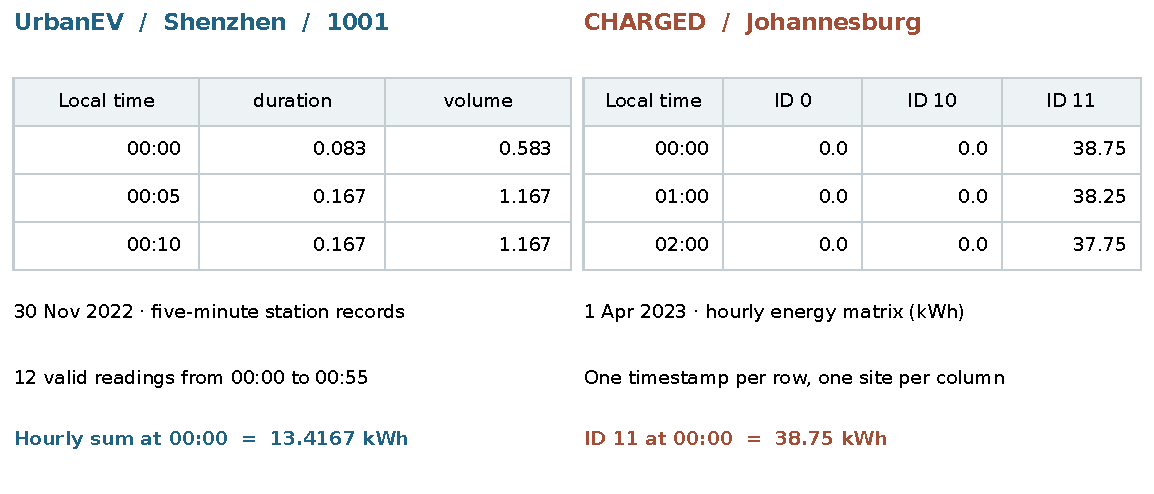
\includegraphics[width=.98\linewidth]{Images/published-records.pdf}
\caption{Published charging records and their hourly interpretation.}\label{fig:published-records}
\end{figure}

An entity key comprises dataset, city and local identifier. UrbanEV/SZH and CHARGED/SZH each have their own source population and target split. All pretraining and subsequent transfer take place within the same dataset and city. Within each group, a salted hash of the dataset, city and local identifier assigns each identifier to exactly one partition. The hash thresholds allocate approximately 60\% to Source, 20\% to Development and 20\% to Final before eligibility screening. Physical correspondence between identifiers in separate releases remains uncertain.

\section{Hourly aggregation and quality control}
For UrbanEV, the hourly total is the sum of twelve consecutive five-minute volume values. The producer requires twelve unique timestamps on the expected grid and finite, nonnegative volume and duration at each timestamp. Duration supplies a validity check. Summing a partially observed hour would systematically understate its energy, so an hour failing this check carries a missing value and a validity flag. CHARGED enters the same hourly interface directly from its released hourly matrix. Both pipelines retain the entity key, timestamp, energy in kWh and file-validity information.

\section{Partitions and target histories}
The source partition supplies established-location training examples. Table~\ref{tab:scope} counts identifiers eligible at 14 days in each partition. Readiness requires a defined entity scale. At this budget, 131 UrbanEV identifiers have undefined scales across the three partitions. To simulate cold start, each experiment restricts the history initially available at a target. The start of this history need not coincide with the opening date of the site.

\begin{table}[htbp]\centering\small
\caption{Entity inventory and eligible identifiers at 14 days.}\label{tab:scope}
\begin{tabular}{lrrrr}\toprule
 & &\multicolumn{3}{c}{Eligible identifiers}\\
\cmidrule(lr){3-5}
Group & Inventory & Source & Development & Final\\\midrule
UrbanEV/SZH &1682&914&296&341\\
CHARGED/AMS &2449&1496&475&478\\
CHARGED/JHB &47&26&8&13\\
CHARGED/LOA &229&137&51&41\\
CHARGED/MEL &63&34&14&15\\
CHARGED/SPO &47&29&8&10\\
CHARGED/SZH &1445&886&288&271\\\bottomrule
\end{tabular}\end{table}

\begin{table}[htbp]\centering\small
\caption{Target cohorts used in the reported comparisons.}\label{tab:target-cohorts}
\begin{tabular}{llrr}\toprule
Comparison & Partition & Selected IDs & History (days)\\\midrule
Backbone benchmark & Development & 4 & 14\\
Calibrated transfer comparison & Development & 12 & 7, 14, 28\\
Historical evaluation & Final & 90 & 7, 14, 28\\
Follow-up evaluation & Development & 46 & 14\\\bottomrule
\end{tabular}\end{table}

UrbanEV stations 1153, 1405, 1693 and 2152 served in both the backbone benchmark and coefficient calibration. Twelve other stations supplied the transfer comparison. The historical Final cohort included 30 UrbanEV identifiers and ten from each CHARGED group. UrbanEV identifier 2193 had no scored outcome. Crossing seven dataset--city groups with three history budgets yielded 21 comparison groups. Seeds 42, 43 and 44 repeated runs on the same entity data. Later exploratory comparisons revisited these Final outcomes.

For the follow-up comparison, the team excluded identifiers with recorded prior use, required at least one complete initial training example, and fixed the cohort before examining its outcomes. In the row order of Table~\ref{tab:scope}, the seven groups contributed 10, 10, 1, 10, 4, 1 and 10 targets. This comparison evaluates additional Development targets at 14 days. Within each group, eligible IDs were ranked by the SHA-256 hash of the study identifier, group and local ID. The first ten were selected, or all eligible IDs when fewer than ten remained. The exclusion audit covers recorded use, and the evaluation shares calendar dates with earlier experiments.

\section{From an hourly series to a forecast example}
For a target with valid observations in its permitted prefix, the energy scale is the 95th percentile of available valid hourly energy using linear interpolation. A zero percentile uses a scale of one. An empty valid prefix leaves the scale undefined and blocks forecasting. The fitted scale remains fixed through replay. For an observed hour, the energy feature is energy divided by this scale and the observation mask equals one. Missing or unavailable historical energy uses a zero placeholder with mask zero. Thus an observed zero and a missing observation produce different inputs.

The historical input has shape \(24\times7\): normalized energy, sine and cosine of local hour, sine and cosine of weekday, a weekend indicator and the energy mask. The forecast-day calendar has shape \(24\times5\) and contains only the calendar channels. An entirely missing history prevents issuance. The 24 future energy values are stored separately with their validity and availability times. A forecast can be scored and used for learning once all 24 labels have arrived and are valid. The same origins must be eligible for both methods in a paired comparison.

Figure~\ref{fig:forecast-tensors} shows the actual feature arrays for the first forecast in the example below. Hour encodings vary within each column over the day. Weekday and weekend features remain constant within each local day. On the history side, the mask stays at one even during hours of zero recorded demand.

\begin{figure}[htbp]\centering
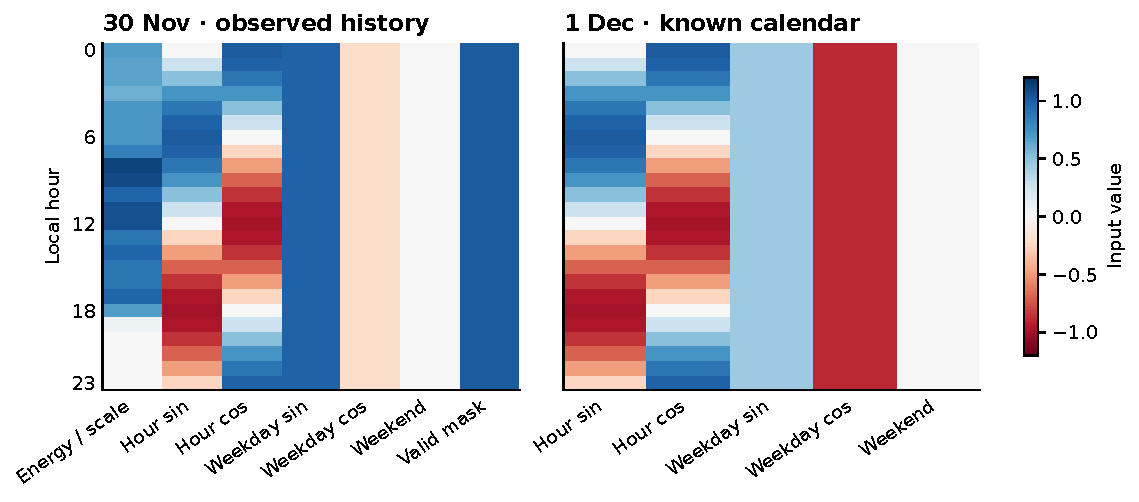
\includegraphics[width=.98\linewidth]{Images/forecast-tensors.pdf}
\caption{Feature arrays supplied to the GRU and forecast head.}\label{fig:forecast-tensors}
\end{figure}

\section{Worked example: UrbanEV station 1001}
The 14-day Development record for station 1001 begins its fit window at midnight on 17 November 2022, Shenzhen time. All 336 prefix hours are valid, including 90 observed zeros. The resulting scale is 19.9792 kWh and 13 complete initial training examples are available. Each pairs one full day of history with the following day of labels; the first pair uses 17 November to forecast 18 November and the last uses 29 November to forecast 30 November. At midnight on 1 December, the historical tensor spans 30 November and the calendar tensor describes 1 December. Figure~\ref{fig:window} displays the corresponding hourly values.



\begin{figure}[htbp]\centering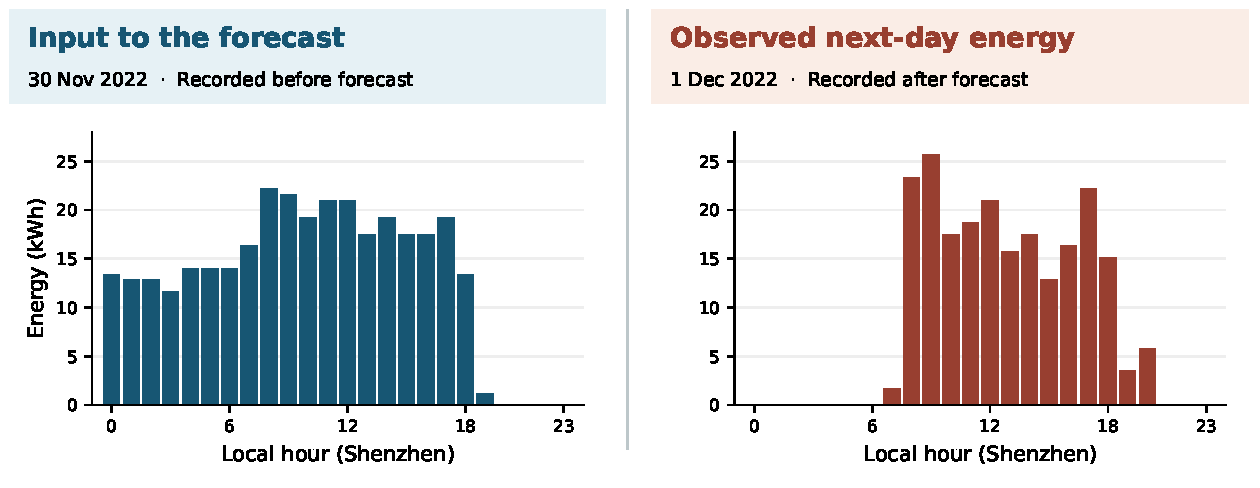
\includegraphics[width=.95\linewidth]{Images/station1001-window.pdf}
\caption{Input history and observed next-day energy at station 1001.}\label{fig:window}
\end{figure}

At 00:00 on 30 November the normalized input is 0.67153, corresponding to approximately 13.42 kWh, with mask one. The released target series on 1 December records zero energy at 06:00 and 1.75 kWh at 07:00. Both values contribute to the eventual score. The label for the final hour becomes available at midnight on 2 December under the replay clock. This example explains the timing of an input and its labels; Figure~\ref{fig:window} plots observations on both sides of the origin.

\par\penalty-200\begingroup\interlinepenalty=10000 Across the 90 requested daily origins for this identifier, 31 have entirely missing histories and 59 produce forecast inputs. Of these, 52 have complete label vectors for evaluation. Figure~\ref{fig:replay-coverage} locates these outcomes on the replay calendar, including the seven issued forecasts with incomplete labels. \par\endgroup

\begin{figure}[htbp]\centering
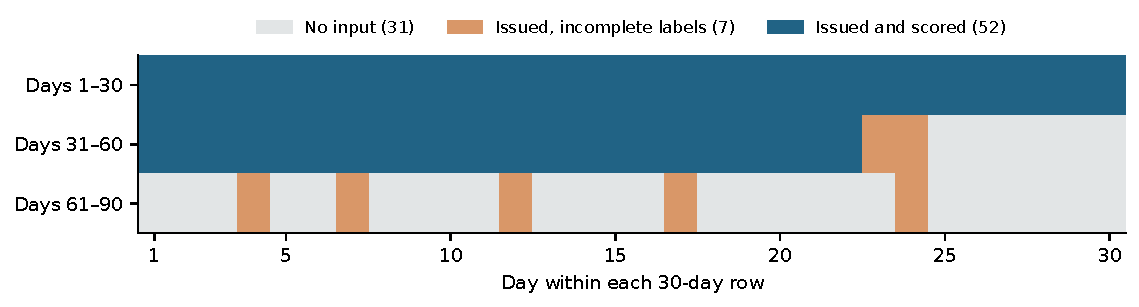
\includegraphics[width=.98\linewidth]{Images/replay-coverage.pdf}
\caption{Daily forecast availability at station 1001.}\label{fig:replay-coverage}
\end{figure}

\begin{figure}[htbp]\centering
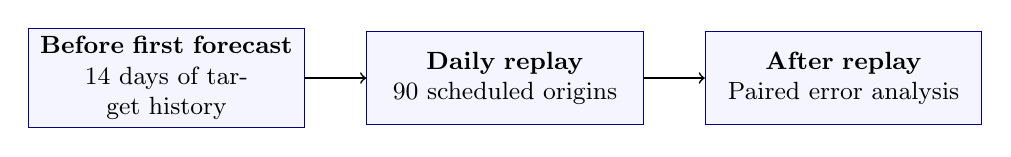
\begin{tikzpicture}[x=1cm,y=1cm]
\tikzset{stage/.style={draw=blue!50!black,fill=blue!4,align=center,text width=3.3cm,minimum height=1.18cm,inner sep=3pt,font=\small}}
\node[stage] (a) at (0,0) {\textbf{Before first forecast}\\14 days of target history};
\node[stage] (b) at (4.3,0) {\textbf{Daily replay}\\90 scheduled origins};
\node[stage] (c) at (8.6,0) {\textbf{After replay}\\Paired error analysis};
\draw[->,semithick](a.east)--(b.west);
\draw[->,semithick](b.east)--(c.west);
\end{tikzpicture}
\caption{Timeline for the locked 46-target evaluation.}\label{fig:locked-timeline}
\end{figure}

In Figure~\ref{fig:locked-timeline}, forecasts precede the next day's observations. The paired analysis uses seven-day calendar blocks, with three- and fourteen-day sensitivity checks. All 36 CHARGED targets had 90 scored days. UrbanEV coverage ranged from 51 to 90 days. Each target mean describes its observed days; the cause of missing observations is unknown.
